Consider the following unity gain feedback system
\begin{center}
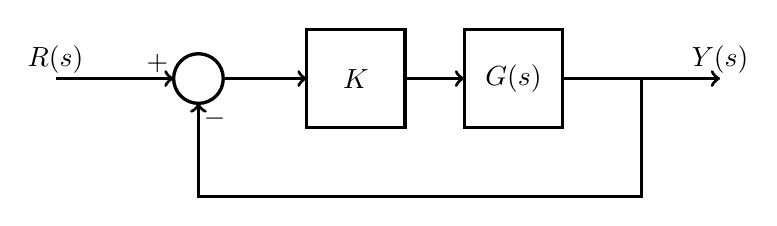
\begin{tikzpicture}[scale=1,inner sep=0pt,outer sep=0pt,very thick,
sysblock/.style={draw,rectangle,inner sep=4pt,minimum width=1.25cm,minimum height=1.25cm,very thick}]

\draw (-2,0) node[draw,circle] (sum1) {$\rule{0pt}{18pt}$};
\draw (0,0) node[sysblock] (C) {$K$};
\draw (2,0) node[sysblock] (G) {$G(s)$};
\draw[<-] (sum1.180) node[above left=2pt] {$+$} -- ++(-1.5,0) node[above=2pt] {$R(s)$};
\draw[->] (sum1.0) -- (C.180);
\draw[->] (C.0) -- (G.180);
\draw[->] (G.0) --  ++(2,0) node[above=2pt] {$Y(s)$};
\draw[->] (G.0) -- ++(1,0) -- ++(0,-1.5) -| (sum1.-90) node[below right=2pt] {$-$};
\end{tikzpicture}
\end{center}
If the following is the Bode plot of $G(s)$, select a gain $K$ so that the closed loop step response rise time is approximately 0.1 s. What is your estimate of the overshoot for the closed loop step response?
\begin{center}
\includegraphics[width=6in]{\mainfolder/LectureNotes/\lecturefolder/HomeworkProblems/Problem01/bode2.pdf}
\end{center}
